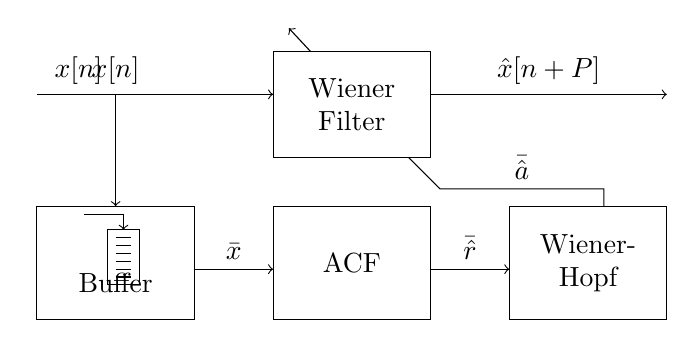
\begin{tikzpicture}

%% Boxes
\draw  (-3,3) rectangle node[text width=2cm,align=center] {Wiener Filter}(-1,4.34);
\draw  (-1,2.38) rectangle node[text width=2cm,align=center] {ACF}(-3,0.94);
\draw  (-4,2.38) rectangle node[text width=2cm,align=center,below=.25] {Buffer}(-6,0.94);
\draw  (0,2.38) rectangle node[text width=1.5cm,align=center] {Wiener- Hopf}(2,0.94);



%%Buffer
\draw (-4.7,1.38) node (v1) {} -- (-5.1,1.38) -- (-5.1,2.08) -- (-4.7,2.08) -- (-4.7,1.38);
\draw (-5,1.98) -- (-4.8,1.98);
\draw (-5,1.88) -- (-4.8,1.88);
\draw (-5,1.78) -- (-4.8,1.78);
\draw (-5,1.68) -- (-4.8,1.68);
\draw (-5,1.58) -- (-4.8,1.58);
\draw (-5,1.48) -- (-4.8,1.48);
\draw [->](-5.4,2.28) -- (-4.9,2.28) -- (-4.9,2.08);


%% Lines
\draw [->](-4,1.58) -- node[above]{$\bar{x}$} (-3,1.58);
\draw [->](-1,1.58) -- node[above]{$\bar{\hat{r}}$}(0,1.58);
\draw (1.2,2.38) -- (1.2,2.6) -- node[above]{$\bar{\hat{a}}$} (-0.88,2.6) -- (-1.28,3);


\draw [->](-2.52,4.34) -- (-2.8,4.64);
\draw [->](-6,3.8) node[right=15,above]{$x[n]$} -- (-3,3.8);
\draw [->](-5,3.8) node[above]{$x[n]$} -- (-5,2.38);
\draw [->](-1,3.8) --  node[above]{$\hat{x}[n+P]$}(2,3.8);
\end{tikzpicture}